\section{方法}

\subsection{数据与任务}

我们使用 JIGSAWS 官方发布版中的缝合（Suturing）任务。元数据文件列出了来自八位外科医生（用户 B 至 I）的 \NTrials{} 个试次。每位用户完成五个试次，只有用户 H 例外：其试次 H002 在官方发布版中没有标签和折划分条目，因此缺失。预测目标是自报技能等级：新手（N，机器人操作经验少于 10 小时）、中级（I，10 至 100 小时）或专家（E，超过 100 小时）。用户 B、G、H、I 为新手（19 个试次），C 和 F 为中级（10 个试次），D 和 E 为专家（10 个试次）。每个试次提供 30\,Hz 采样的 76 个运动学通道，即两个医生端主控臂和两个患者端器械各自的笛卡尔位置、旋转矩阵、线速度、角速度和夹钳角度，以及两路 640$\times$480 像素、每秒 30 帧的内窥镜视频。运动学特征只使用患者端器械，因为它们是真正作用于组织的工具，而在遥操作下主控臂信号与之高度重复；视频特征使用左侧相机视图（capture1）。试次时长在 \DurMin{} 至 \DurMax{}\,s 之间（中位数 \DurMedian{}\,s），新手平均更慢（图~\ref{fig:data}）。任何模型都不使用手势标注或 OSATS 评分。

\begin{figure}[htbp]
\centering
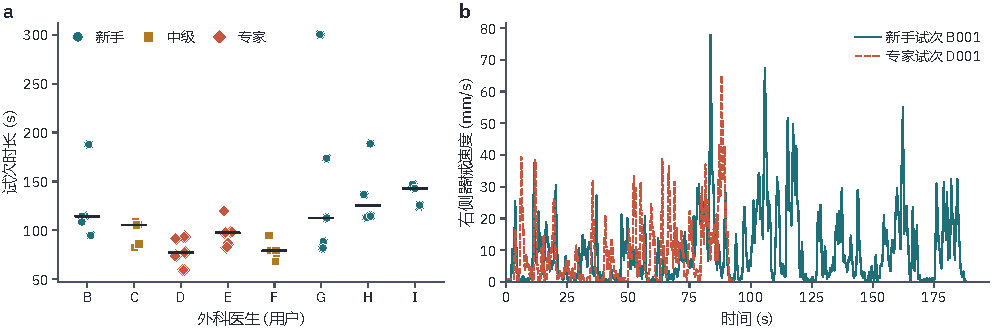
\includegraphics{fig2_data_zh.pdf}
\caption{(a) 各外科医生的试次时长，颜色表示技能等级，横线为中位数。(b) 一个新手试次（B001）和一个专家试次（D001）中右侧患者端器械的速度（0.5\,s 平滑）。专家用约一半的时间完成任务，峰值速度相近。}
\label{fig:data}
\end{figure}

\subsection{工作流程}

图~\ref{fig:pipeline} 概括了整个流程。每个试次被转换为若干定长特征向量，每个特征块对应一个向量。每个特征块由标准化后的 L2 正则逻辑回归分类，其正则化强度在训练外科医生内部选择。多模态模型要么在分类前拼接特征块（早期融合），要么对一个运动学分类器和一个视频分类器的类别概率取平均（后期融合）。所有模型都在 JIGSAWS 技能检测设置的八个官方 LOUO 折上评估。

\begin{figure}[htbp]
\centering
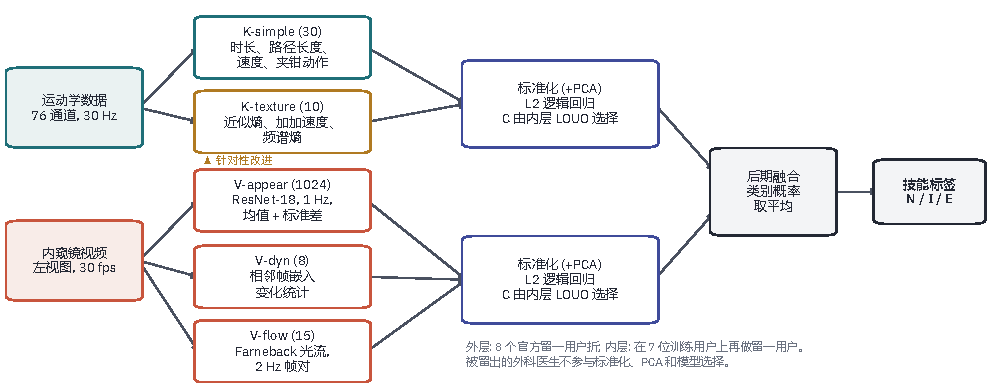
\includegraphics{fig1_pipeline_zh.pdf}
\caption{工作流程。每个试次提取运动学和视频特征块，由正则化逻辑回归分类；后期融合对一个运动学分类器和一个视频分类器的类别概率取平均。K-texture 特征块是本文的针对性改进。括号内数字为特征维数。所有拟合步骤（包括标准化、PCA 和正则化强度的选择）都只使用每一折的训练外科医生。}
\label{fig:pipeline}
\end{figure}

\subsection{运动学特征}

仅运动学基线（K-simple，30 维）实现了任务说明中点名的统计量。对每个患者端器械，我们计算：路径长度（相邻工具尖端位置间距离之和）；线速度的均值、标准差和第 90 百分位数；角速度的均值和标准差；静止比例，即线速度低于 5\,mm/s 的采样点所占比例；运动经济性，即路径长度除以工具尖端轨迹包围盒的对角线长度；以及五个夹钳统计量，即夹钳角度的均值、标准差、范围、总绝对变化量和开合次数（以 0.5\,s 滑动平均信号向上穿越其均值的次数计）。另有四个试次级特征：时长（秒）、两个器械速度之间的相关系数、两者同时静止的时间比例，以及两条路径长度之比的对数。这些都是描述效率和双手协调的常用指标\citep{reiley2011review, lefor2020motion}。

运动纹理特征块（K-texture，10 维）是本文的针对性改进，参照背景文献\citep{zia2018rmis}设计。对每个器械，我们计算线速度、角速度和夹钳角度的近似熵\citep{pincus1991apen}（均重采样到 10\,Hz，嵌入维数 $m = 2$，容差 $r$ 取信号标准差的 0.2 倍）；速度曲线的对数无量纲加加速度（log dimensionless jerk）\citep{hogan2009smoothness}；以及速度的归一化频谱熵。这些特征描述的是动作有多规律、多平滑，而不是多快或多长；按设想，即使两人用时相近，这一性质也应能区分动作流畅的专家和犹豫不决的新手。

\subsection{视频特征}

每个试次的视频只解码一遍。每 30 帧取一帧（1\,Hz，共 \NFramesOneHz{} 帧），缩放到 224$\times$224 像素后输入去掉分类层的 ImageNet 预训练 ResNet-18\citep{he2016resnet}，得到每帧 512 维嵌入。外观特征块（V-appear，1024 维）是这些嵌入在整个试次上的均值和标准差；由于 1024 维对 34 个训练试次而言维数过高，我们在每个训练折内拟合 4、8 或 16 个主成分的 PCA。场景动态特征块（V-dyn，8 维）概括画面变化的快慢：由相邻 1\,Hz 嵌入之间的余弦距离取均值、标准差、第 10/50/90 百分位数和变异系数，由欧氏距离取均值和标准差。某一录制场次中恒定的外观成分（例如光照或练习板的摆放）在差分中相互抵消，因此 V-dyn 携带的录制环境信息应少于 V-appear，同时仍能反映器械运动和组织变化。光流特征块（V-flow，15 维）在以 2\,Hz 采样、缩放到 320$\times$240 像素的相邻帧对（共 \NPairsTwoHz{} 对）上计算 Farneback 稠密光流\citep{farneback2003flow}。对每个帧对，我们计算光流幅值的均值、标准差和第 90 百分位数、运动速度超过每帧 0.5 像素的像素比例，以及按幅值加权的 8 方向光流方向熵；这五个序列再分别用试次内的均值、标准差和第 90 百分位数概括。

\subsection{分类器与融合}

所有特征块使用同一模型：标准化、可选的 PCA（仅 V-appear）、PCA 后再次标准化，以及带 L2 惩罚、类别平衡权重和 L-BFGS 求解器的多项逻辑回归\citep{pedregosa2011sklearn}。逆正则化强度 $C$ 从 $\{0.01, 0.03, 0.1, 0.3, 1, 3, 10\}$ 中选择，V-appear 的主成分数从 $\{4, 8, 16\}$ 中选择。后期融合以相等权重平均运动学分类器和一个视频分类器的类别概率；采用等权重是因为 34 个训练试次不足以可靠地估计融合权重。早期融合把 K-simple 与 V-dyn 拼接后拟合一个分类器。主多模态模型在看到任何结果之前就已确定，即 K-simple 与 V-dyn 的后期融合（M3）。选择 V-dyn 作为主视频特征块，一是出于上面所述的基本原理，二是因为本组此前在同样 39 个试次上的探索性分析发现嵌入变化统计量是最有希望的视频描述符。由于那次分析看过同一数据上的折外结果，这一选择并非完全不受选择偏差影响，因此我们报告全部三个视频特征块和全部四种融合变体。

\subsection{评估协议}

我们使用 \texttt{Suturing/unBalanced/SkillDetection/UserOut} 中的 JIGSAWS 官方折；代码检查每一折恰好留出一位外科医生，共八折，每折训练试次为 34 或 35 个。超参数由每个外层折内、在七位训练外科医生上进行的内层 LOUO 循环选择，以内层合并 macro-F1 最大为准，平局时取更强的正则化。当外层折留出的是中级或专家外科医生时，该类只剩一位外科医生，内层留出它的那一折就没有该类的训练样本；这样的内层折被跳过（每个受影响的外层折跳过一个）。因此被留出的外科医生从不影响标准化、PCA、特征残差化或模型选择。

主要指标是在 39 个合并的折外预测上一次性计算的 macro-F1。由于标签在同一外科医生内部恒定，每个 LOUO 测试折只含一个类别，另外两个缺失类别的逐折 macro-F1 没有定义，所以合并计算是该指标唯一良好定义的形式。我们同时报告准确率、各类别 F1、混淆矩阵和每位外科医生的准确率。只有八位外科医生时不确定性很大，因此我们用两种尊重试次分组结构的方法加以量化。用户级 bootstrap 对八位外科医生有放回地重采样 2000 次，给出 macro-F1 及模型间配对差值的百分位区间。精确置换检验在外科医生之间重新分配技能标签，同时保持每位外科医生的试次在一起；四位新手、两位中级、两位专家共有 $8!/(4!\,2!\,2!) = 420$ 种不同的分配方式，因此固定预测下 macro-F1 的零分布可以被精确枚举，可达到的最小 $p$ 值为 $1/420$。我们事先声明了三个比较：运动学对多数类（M1 对 M0）、在运动学上加入视频（M3 对 M1）、加入运动纹理（M4 对 M1）。只有当 bootstrap 区间不包含零时，才认为差异得到支持。完整协议（包括表~\ref{tab:main} 中的模型列表）在流程运行之前写入 \texttt{PROTOCOL.md}，每个模型只评估一次。

\subsection{捷径审计}

这里可能存在两类捷径。其一，特征块可能识别出外科医生身份，这时分类器可以通过“认人”复现训练标签，而这种能力无法迁移到新的外科医生。我们用身份探针测量这一点：在每个特征块上训练一个八分类的外科医生识别器，用按试次分层的五折交叉验证评估，并将其平衡准确率与随机水平 1/8 比较。其二是节奏。新手平均更慢，模型可能只是按时长给试次排序，却被当作技能。我们用仅时长分类器（C1），以及把每个特征对 log 时长做残差化后的 K-simple（C2；加入纹理特征后为 C2t）来检验，其中回归只在训练外科医生上拟合。

\subsection{与已有工作的区别}
\label{sec:differences}

与背景文献和大多数相关工作相比，我们的方法有四点不同。第一，报告的数字来自运行前就固定的协议：所有模型、指标和比较都事先写明，每个模型只评估一次，因此最终报告哪个模型不可能取决于测试结果。第二，我们把八位外科医生而不是 39 个试次作为不确定性的基本单位，报告用户级 bootstrap 区间和覆盖全部 420 种标签分配的精确置换检验，而不是单一的准确率；并使用 macro-F1，使两个小类别与新手类同等重要。第三，我们直接测量两种捷径，即每个特征块携带的外科医生身份信息，以及决策中可由试次时长解释的部分，而不是默认高分就代表技能。第四，场景动态描述符 V-dyn 的设计目的是抵消录制场次的静态外观（整帧外观特征保留了这部分信息），我们也直接检验了它是否减弱了身份捷径。

\subsection{外部资源与本组工作}

我们使用了 JIGSAWS 数据及其官方划分文件、torchvision 提供的 ResNet-18 ImageNet 权重\citep{paszke2019pytorch}、OpenCV 中的 Farneback 实现\citep{bradski2000opencv}，以及用于分类器和信号处理的 scikit-learn\citep{pedregosa2011sklearn}、NumPy\citep{harris2020numpy} 和 SciPy\citep{virtanen2020scipy}。没有使用任何已发布的技能评估代码。数据读取与折校验、全部特征定义、嵌套 LOUO 评估、融合模型、bootstrap 与精确置换分析、捷径审计以及所有图表均由本组实现。
